\chapter{Codifica}

\section{Tecnologie e strumenti}

\subsection{Linguaggio e piattaforma}
Il \textit{middleware} è stato sviluppato in \nameref{Java} e gestito tramite \nameref{Apache Maven} come \textit{build tool}, che si occupa della risoluzione delle dipendenze, della compilazione e del \textit{packaging} dell'applicazione in un \textcolor{purple}{jar} eseguibile.

\subsubsection{Java}
\label{Java}
Java è un linguaggio di programmazione ad alto livello, orientato agli oggetti e a tipizzazione statica, che si appoggia sull'omonima piattaforma \textit{software} di esecuzione, specificamente progettato per essere il più possibile indipendente dalla piattaforma \textit{hardware} di esecuzione (tramite compilazione in \textit{bytecode} prima e interpretazione poi da parte di una \acrshort{JVM}).
\begin{figure}[H]
    \centering
    
\includegraphics[width=0.2\textwidth]{assets/java.png}
    \caption{Java}
\end{figure}

\subsubsection{Apache Maven}
\label{Apache Maven}
Apache Maven è uno strumento di gestione di progetti \textit{software} basati su \nameref{Java} e \textit{build automation}. \\
Maven usa un costrutto conosciuto come \acrshort{POM}; un file \acrshort{XML} che descrive le dipendenze fra il progetto, le varie versioni di librerie necessarie e le dipendenze fra di esse. In questo modo si separano le librerie dalla \textit{directory} di progetto utilizzando questo file descrittivo per definirne le relazioni. \\
Maven effettua automaticamente il \textit{download} di librerie \nameref{Java} e \textit{plug-in} Maven dai vari \textit{repository} definiti scaricandoli in locale o in un \textit{repository} centralizzato lato sviluppo. Questo permette di recuperare in modo uniforme i vari file \acrshort{JAR} e di poter spostare il progetto indipendentemente da un ambiente all'altro avendo la sicurezza di utilizzare sempre le stesse versioni delle librerie.
\begin{figure}[H]
    \centering
    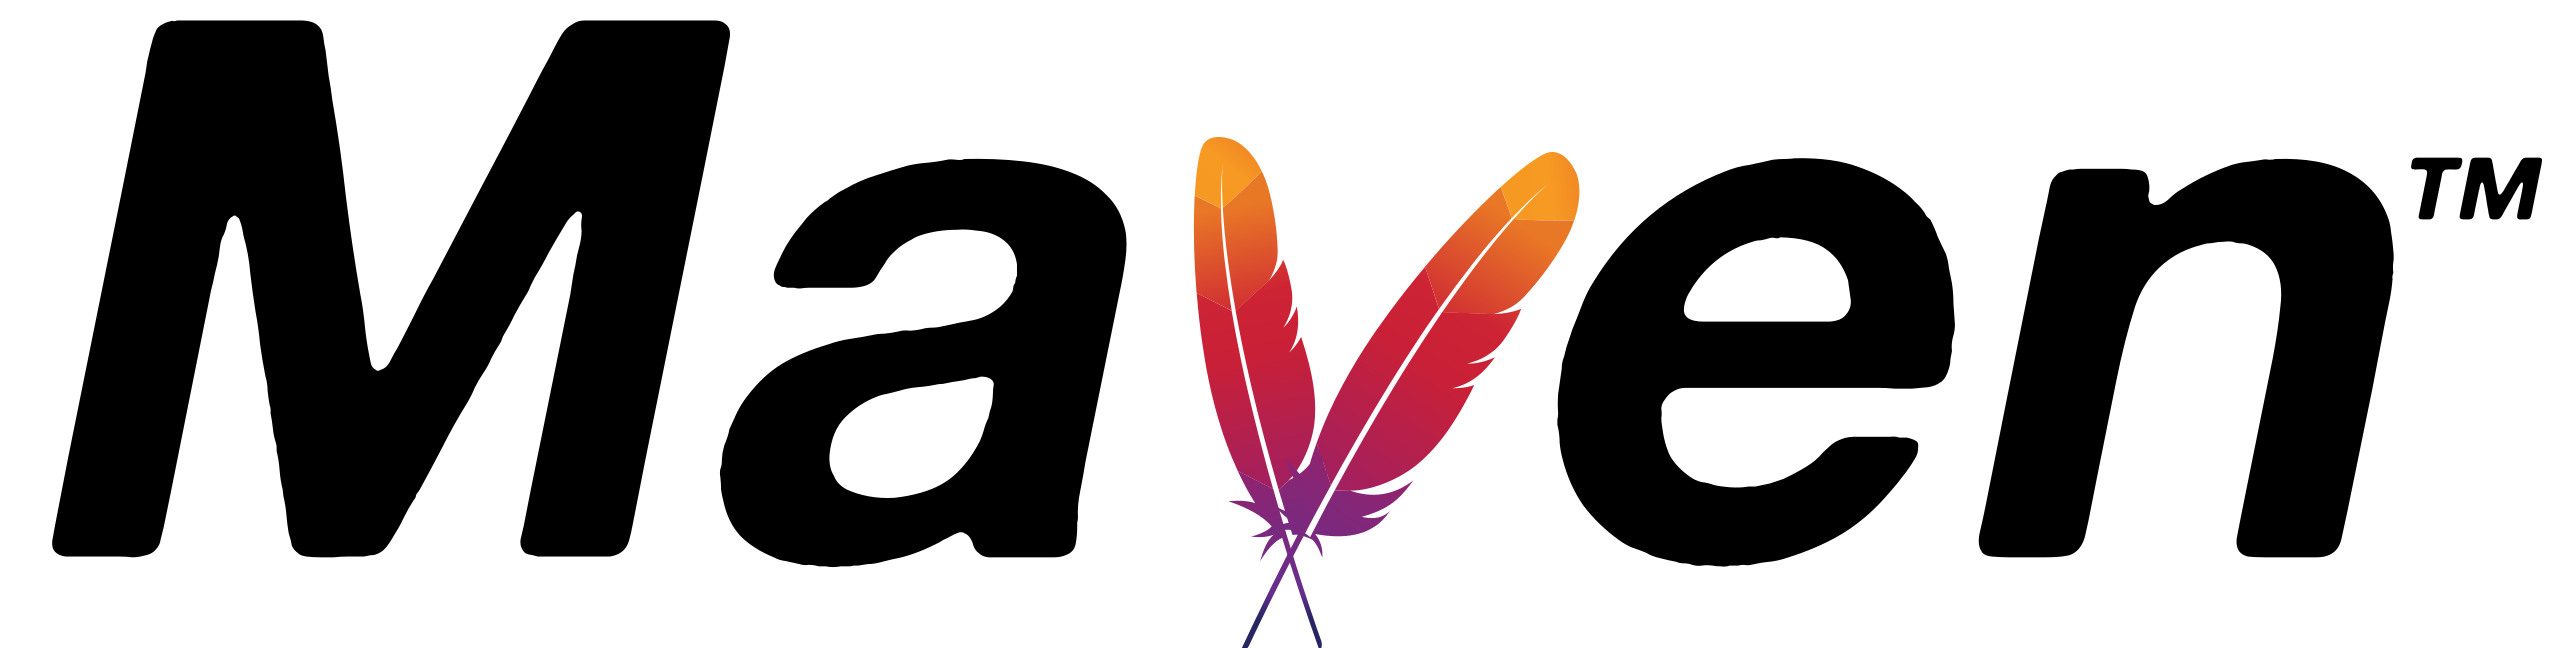
\includegraphics[width=0.4\textwidth]{assets/apacheMaven.png}
    \caption{Apache Maven}
\end{figure}

\subsection{Framework applicativo}
Il progetto si basa principalmente sul framework Spring, in particolare i seguenti moduli:
\begin{itemize}
    \item \textbf{Spring Boot:} per semplificare la configurazione e l'avvio di applicazioni Java
    \item \textbf{Spring Data JPA:} per la persistenzadei dati
    \item \textbf{Spring Kafka:} per l'integrazione dichiarativa con \nameref{Apache Kafka} (consumer, producer, listener)
\end{itemize}

\subsubsection{Spring}
\label{Spring}
Spring è un framework \gls{Open Source} per lo sviluppo di applicazioni su piattaforma Java.
A questo framework sono associati tanti altri progetti, che hanno nomi composti come Spring Boot, Spring Data JPA e Spring Kafka. 
Questi progetti sono stati ideati per fornire funzionalità aggiuntive al framework.
\begin{figure}[H]
    \centering
    
\includegraphics[width=0.4\textwidth]{assets/spring.png}
    \caption{Spring}
\end{figure}

\subsection{Infrastruttura di supporto}
L'ambiente di sviluppo è orchestrato tramite Docker e Docker Compose, secondo la definizione riportata nel file \textcolor{purple}{docker-compose.yml}, che avvia tre servizi containerizzati:
\begin{itemize}
    \item \textbf{PostgreSQL:} il \textit{database} relazionale che ospita i dati di arricchimento;
    \item \textbf{Apache Kafka:} configurato in modalità KRaft (Kafka Raft), l'architettura più recente che elimina la dipendenza da Apache ZooKeeper per il coordinamento del \textit{cluster}, unificando i ruoli di \textit{broker} e \textit{controller} in un singolo nodo (scelta adeguata a un ambiente di sviluppo locale a singolo nodo);
    \item \textbf{Kafka UI:} un'interfaccia web (esposta sulla porta \textcolor{purple}{8081}) che consente di ispezionare topic, partizioni, messaggi e \textit{consumer group} senza dover ricorrere alla sola riga di comando.
\end{itemize}
Questa infrastruttura consente di riprodurre in locale, in modo rapido e ripetibile, un ambiente rappresentativo di un \textit{deployment} di produzione, mantenendo però la semplicità necessaria in fase di sviluppo e test.

\subsubsection{Docker}
\label{Docker}
Docker è un popolare \textit{software} libero che utilizza la virtualizzazione a livello di sistema operativo per eseguire applicazioni in ambienti isolati chiamati \textit{container}. \\
I container Docker sono un'estensione dei \textit{container} del sistema operativo. Docker supporta sia i container Linux che quelli Windows. È possibile utilizzare Docker con container Linux anche nei sistemi Windows e MacOS grazie a tecniche di virtualizzazione.
\begin{figure}[H]
    \centering
    
\includegraphics[width=0.4\textwidth]{assets/docker.png}
    \caption{Docker}
\end{figure}

\subsubsection{PostgreSQL}
\label{PostgreSQL}
PostgreSQL è un completo \acrshort{DBMS} ad oggetti pubblicato con licenza libera (stile Licenza BSD). Spesso abbreviato come "Postgres", sebbene questo sia un nome vecchio dello stesso progetto, è una reale alternativa sia rispetto ad altri prodotti liberi come MySQL, Firebird SQL e MaxDB che a quelli a codice chiuso come Oracle, IBM Informix o DB2 ed offre caratteristiche uniche nel suo genere che lo pongono per alcuni aspetti all'avanguardia nel settore delle basi di dati. 
\begin{figure}[H]
    \centering
    
\includegraphics[width=0.3\textwidth]{assets/postgresql.png}
    \caption{PostgreSQL}
\end{figure}

\subsubsection{Apache Kafka}
\label{Apache Kafka}
Apache Kafka è una piattaforma \gls{Open Source} di \textit{stream processing} scritta in Java e Scala e sviluppata dall'Apache Software Foundation. Il progetto mira a creare una piattaforma a bassa latenza ed alta velocità per la gestione di \textit{feed} dati in tempo reale. \\
Questo progetto viene usato principalmente per tutte le applicazioni di elaborazioni di \textit{stream} di dati in tempo reale.
\begin{figure}[H]
    \centering
    
\includegraphics[width=0.4\textwidth]{assets/apacheKafka.png}
    \caption{Apache Kafka}
\end{figure}

\section{Progettazione}
\label{Progettazione}
Prima di procedere all'implementazione, sono state definite alcune scelte progettuali riguardanti il modello dei dati, la struttura dei \gls{Topic Kafka} e la gestione degli errori.

\subsection{Modello dei dati}
Sono stati definiti tre tipi di oggetti, ciascuno con una responsabilità precisa:
\begin{itemize}
    \item \textcolor{purple}{OrderEvent}: rappresenta il messaggio grezzo in ingresso, contenente un identificativo dell'ordine (\textcolor{purple}{orderId}), un riferimento al cliente (\textcolor{purple}{customerId}) e i dati dell'ordine stesso (\textcolor{purple}{product}, \textcolor{purple}{amount});
    \item \textcolor{purple}{Customer}: entità contenente i dati del cliente (\textcolor{purple}{fullName}, \textcolor{purple}{email}, \textcolor{purple}{city}) necessari all'arricchimento;
    \item \textcolor{purple}{EnrichedOrder}: rappresenta il messaggio finale pubblicato in uscita, che unisce i dati dell'ordine originario con i dati del cliente recuperati da \nameref{PostgreSQL}, più un \textit{timestamp} (\textcolor{purple}{enrichedAt}) che documenta il momento dell'arricchimento.
\end{itemize}
Questa separazione segue il pattern \nameref{Content Enricher}: il messaggio in ingresso è  "povero", mentre il contratto in uscita è "arricchito" con informazioni che il produttore originario dell'evento non possiede.

\subsection{Progettazione dei topic Kafka}
Sono stati previsti tre topic, ciascuno con un numero di partizioni proporzionato al ruolo previsto:
\begin{table}[H]
    \setlength{\tabcolsep}{10pt} % Default value: 6pt
    \def\arraystretch{1.5} % Default value: 1
    \centering
    \begin{tabular}{|l|l|p{0.45\linewidth}|}
        \hline
        \textbf{Topic} & \textbf{Partizioni} & \textbf{Ruolo} \\ \hline
        \textcolor{purple}{orders-input} & 3 & ingresso degli ordini grezzi \\ \hline
        \textcolor{purple}{orders-output} & 3 & uscita degli ordini arricchiti \\ \hline
        \textcolor{purple}{orders-input-dlq} & 1 & dead letter queue per ordini non arricchibili \\ \hline
    \end{tabular}
    \caption{Tabella dei topic}
    \label{Tabella dei topic}
\end{table}
\noindent
Il numero di partizioni maggiore per i topic di flusso principale (\textcolor{purple}{orders-input}, \textcolor{purple}{orders-output}) consente il parallelismo in lettura/scrittura descritto in \ref{Event Streaming}.
La singola partizione per la \acrshort{DLQ} riflette invece un volume atteso più basso e la priorità data alla semplicità di ispezione rispetto al parallelismo.

\subsection{Progettazione del flusso di elaborazione}
Il flusso di elaborazione è stato progettato secondo la seguente sequenza logica:
\begin{enumerate}
    \item un evento ordine viene pubblicato su \textcolor{purple}{orders-input};
    \item il middleware consuma il messaggio;
    \item il middleware tenta di recuperare i dati del cliente corrispondente su \nameref{PostgreSQL};
    \begin{enumerate}
        \item se il cliente viene trovato, viene composto il messaggio arricchito e pubblicato su \textcolor{purple}{orders-output};
        \item se il cliente non viene trovato, l'evento originario viene instradato su \textcolor{purple}{orders-input-dlq}, secondo il pattern \nameref{Dead Letter Channel} descritto in \ref{Dead Letter Channel};
    \end{enumerate}
\end{enumerate}
\begin{figure}[H]
    \centering
    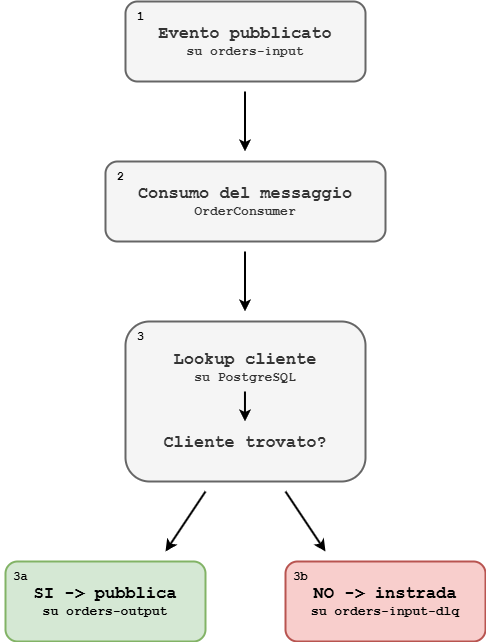
\includegraphics[width=0.5\textwidth]{assets/flusso.drawio.png}
    \caption{Flusso di elaborazione}
\end{figure}
Questa progettazione garantisce che, in caso di arresto anomalo dell'applicazione tra la lettura del messaggio e la sua elaborazione completa, il messaggio venga riletto al riavvio (semantica at-least-once, discussa in \ref{Semantica di consegna}), evitando così perdite di dati a scapito di un'eventuale elaborazione duplicata.

\newpage
